\documentclass[a4paper]{article}

\usepackage[margin=2.5cm]{geometry}
\usepackage{hyperref}
\usepackage{tikz}
\usepackage{listings}
\lstset{frame=single}

\begin{document}

\title{Deployment of SCION on Bare Metal Switches}
\author{Lars-Christian Schulz \and Cecil Benjamin Leonard}

\maketitle

\begin{abstract}
The aim of our project is to explore potential applications of a bare metal switch in SCION packet forwarding. To this end we identify a suitable network operating system and describe how to install SCION on it and assess its performance. We present a number of switch fabric APIs and examine their capabilities regarding their usefulness in a SCION border router. This includes establishing a suitable development environment and testing the limitations imposed by the APIs and the actual hardware with our own applications. This report summarizes the challenges we faced and documents the course of action we took in overcoming them.
\end{abstract}

\tableofcontents

\section{Introduction}
SCION is an internet architecture that is capable of routing control, failure isolation, and explicit trust information for end-to-end communication. A bare-metal switch is a network device without a network operating system. We can decide on an operating system. It is cheaper and features based on the operating system can be customized in comparison to a closed switch. We aim to implement SCION on an Edgecore bare metal switch, test SCION's functionality and know its limitations when implemented in a bare metal switch. Unlike closed switches, a bare metal switch's network operating system can be chosen by the user. We were able to access the Broadcom ASIC API for enabling Ethernet ports in the Linux environment. We had to choose an open source network operating system which supports the right processor architectures. Open Network Linux was used as a network operating system with OpenNSL as switch fabric API. The following chapters will brief about each issue resolved while deploying SCION in bare metal switches.

%%%%%%%%%%%%%%%%%%%%%%%%%%%%%%%

\section{Switch Hardware}
We had two Edgecore bare metal switches available for this project. The first is an AS4610-54T\footnote{\url{https://www.edge-core.com/productsInfo.php?cls=1&cls2=9&cls3=46&id=21}} featuring 48 Gigabit Ethernet ports. It utilizes a Broadcom BCM56340 Helix4 switching ASIC and a dual-core ARM Cortex A9 at 1~GHz with 2~GB of DDR3 SDRAM. The second switch is an AS5812-54T\footnote{\url{https://www.edge-core.com/productsInfo.php?cls=1&cls2=8&cls3=59&id=113}} with 48 10Gb Ethernet ports and a Broadcom BCM56864 Trident2+ ASIC. In contrast to the first switch it has an x86 processor, an Intel Atom C2538 quad-core at 2.4~GHz with 8~GB DDR3 RAM. This means we had two different processor architectures to work with. Additional technical information is summarized in Table~\ref{tab:switch_specs}.

\begin{table}[thb]
\begin{tabular}{l|l|l}
& AS4610-54T & AS5812-T \\
\hline
Ethernet Ports & 48x1~Gbps & 48x10~Gbps \\
Switch Silicon & BCM56340 Helix4 & BCM56864 Trident2+ \\
CPU & ARM Cortex A9 (dual-core, 1~GHz) & Intel Atom C2538 (quad-core, 2.4~GHz) \\
Memory & 2~GB DDR3 EEC DRAM & 8~GB DDR3 EEC DRAM \\
Storage & 8~MB SPI Flash, 8~GB NAND Flash & 16~MB SPI Flash, 8~GB NAND Flash \\
Switching Capacity & 128~Gbps & 1.44~Tbps \\
Forwarding Rate & 131~Mpps & 1~Bpps \\
\end{tabular}
\caption{Key components and performance figures of the switches}
\label{tab:switch_specs}
\end{table}

%%%%%%%%%%%%%%%%%%%%%%%%%%%%%%%

\section{Network Operating Systems}
SCION can run on multiple platforms such as Ubuntu, ARM minicomputers and Android devices. Installing a compatible operating system on the switches was the first step.

We could run a standard Ubuntu distribution on the switches, but the extended networking peripherals of the device would not be supported. A network operating system comes with specific functionalities supporting the bare metal switch hardware unlike the traditional distribution. These are a few network operating systems, e.g, PICA OS, Cumulus OS, Open Network Linux (ONL), and OpenSwitch (OPX). Using an open source operating system for the open hardware switches seemed a better option, because PICA and Cumulus OS require a license for installation and support. As per the switch hardware an operating system that runs on an ARM processor and another that works on an x86 machine is required.

\subsection{Open Network Linux}
We chose Open Network Linux, because it is an open source operating system. It is available for most existing processors. It is Debian based. Debian has three different actively supported ARM ports\footnote{\url{https://www.debian.org/ports/arm/}}: ARM-EABI (armel), ARM-Hard-Float (armhf), and 64-bit ARM (arm64). Since we worked with a 32-bit ARM architecture, only armel and armhf were of interest. The major difference between them is that armhf takes advantage of the hardware floating-point unit build into many modern ARM cores, whereas armel must remain compatible with systems without an FPU potentially degrading floating-point performance. Sine the ARM Cortex A9 we had has an FPU, armhf is expected to work more efficiently.

When we initially considered ONL armhf was not officially supported, so we had to resort to armel for our ARM based switch. Since December 2018 armhf builds are supported and some time later official precompiled binaries were supplied. Before we had the precompiled binaries, we were able to compile ONL following the instructions published in its repository\footnote{\url{https://github.com/opencomputeproject/OpenNetworkLinux/blob/master/docs/Building.md}}.

Open Network Linux does not come with production-ready forwarding code. Third-party binaries can be used for forwarding applications. An open source SDK was available for packet forwarding hardware. Broadcom OF-DPA and OpenNSL SDKs are examples.

We are using Debian 9 armel based ONL as operating system for the AS4610-54T. We settled on the armel port, because Edgecore only provides OF-DPA and OpenNSL binaries for an armel kernel. While the user mode components of these SDKs run on the armhf port, the necessary kernel modules limit out choice of OS. We also tried compiling the kernel modules on our own but ultimately failed, see Section~\ref{sec:kernel_modules}. Debian9 AMD64 based ONL is used as operating system for the AS5812-54T. The steps for deploying ONL can be found in the official GitHub repository\footnote{\url{https://edge-core.github.io/Deployment-Guide-ONL/}}.

\subsection{Open Switch}
Open Switch is based on Debian Jessie. Officially OPX supports a range of x86 DELL EMC and Edgecore network switches as of now\footnote{\url{https://github.com/open-switch/opx-docs/wiki/hardware-support}}. It has ready-to-use switching implementations in contrast to ONL which is intended as a development kit. OPX supports the SAI switch fabric API.

%%%%%%%%%%%%%%%%%%%%%%%%%%%%%%%
\section{Running SCION on Open Network Linux}
We edited the preexisting scion scripts for installation and update to work under Open Network Linux for the ARM based AS4610-54T and the x86 quad core processor of the AS5812-54T.

SCION is an application that is compatible with Ubuntu. Since we use ONL which is Debian based SCION does not run out of the box. It has some dependencies not available in Debian. So we installed a few required packages manually. Some where installed from a backport repository.

SCION was installed on ONL based on the armel port of Debian~9. The hardware used requires armhf, only then the processor can be utilize to its full capacity. SCION was also tested and implemented in the x86 based switch. In the section below we will discuss the issues we overcame while installing SCION in ONL.

\subsection{SCION on armel}
SCION and its dependencies are compatible with Ubuntu environments and ONL is a Debian based operating system.

\paragraph{Installation of SCION in Debian 8 based ONL}
The steps to install SCION are already well documented in the SCION tutorials\footnote{\url{https://netsec-ethz.github.io/scion-tutorials/native_setup/ubuntu_x86_build/}}. We used the existing script as reference and installed SCION manually in Debian. The pip package which is utilized for Python package management was updated. We also updated Python versions from 3.4.2 to 3.5.2. After the update Python~3.5.2 is set as default. SCION patches and packages are cloned from the GitHub.

\paragraph{Installation of Dependencies}
Dependence packages are installed before installing SCION. \texttt{capnproto} and \texttt{libcapnp-dev} packages are unavailable in Debian 8, hence they were installed from Jessie-back ports:
\begin{lstlisting}
sudo apt-get -y -t jessie-backports install capnproto libcapnp-dev
\end{lstlisting}

While installing the required python packages we found that \texttt{flake8}, \texttt{python3-lz4}, \texttt{python3-nacl}, and \texttt{python3-nose-cov} are not compatible with the Debian. Hence we installed \texttt{lz4}, \texttt{PyNaCl}, \texttt{nose-cov}, and \texttt{flake8}. Flake installation failed because of its inter-dependence on \texttt{pyflakes}~1.1, but \texttt{pyflakes}~1.1.0 is incompatible with SCION. The next step was to install \texttt{requests} version~2.9.1 before installing \texttt{sphinxcontrib-napoleon}.

After installing the dependencies installing SCION was successful. Zookeeper was configured later.

\paragraph{Installation of SCION in Debian9 based armhf ONL}
We installed SCION with same steps as we used for Debian~9 and we faced the following issues: Error when installing cryptography, so we upgraded the version of cryptography from 1.8.1 to 1.9 as suggested here: \url{https://github.com/pyca/cryptography/issues/3605}. Version 1.9 did not work either due to an incompatibility with the system's OpenSSL, so we upgraded to version 2.5 and added an explicit dependency on \texttt{pyOpenSSL} version 19.0.0 to SCION's requirements file.

The \texttt{setcap} command failed because the ONL image comes without \texttt{setcap} installed. Installation of \texttt{libcap2-bin} enabled the \texttt{setcap} command.

SCION was unable to find if Docker is running or not due to a kernel feature required by Docker (cgroups) being disabled in the armhf version of ONL.

With these steps we successfully installed SCION in Debian~8 as well as in the Debian~9 based armel image.

%%%%%%%%%%%%%%%%%%%%%%%%%%%%%%%

\subsection{SCION on x86 (Debian 9 based ONL)}
The installation procedure is identical to the installation on the the ARM system, but no errors occur because of disabled kernel features. The kernel configuration ONL uses for x86 platforms seems to be closer the the Debian~9 defaults.

\paragraph{Moving SCION to USB}
After installation of SCION on the internal flash memory of the switch, we found that the log files generated whenever SCION runs will relatively quickly wear out the flash memory cells. Hence we moved the SCION and Zookeeper logs to an external USB drive.

%%%%%%%%%%%%%%%%%%%%%%%%%%%%%%%

\subsection{SCION traffic on a physical loop connection}
After we had a running operating system with SCION on it, we implemented the network configuration. We created virtual network interfaces using the KNET feature of OpenNSL (see Section~\ref{sec:opennsl_test_app}) ASes are configured in the same switch, hence packets are send and received via the Linux network stack. We wanted to transmit and receive from separate network namespaces, so that the communication between two AS can access separate Linux network stacks and packets flow through the physical ports. Below snippet shows how to configure the namespaces and how to add the switch ports to them.
\begin{lstlisting}
sudo ip netns add ns1
sudo ip link set scion1 netns ns1
sudo ip netns exec ns1 ip addr add dev scion1 10.0.8.1/24
sudo ip netns exec ns1 ip link set dev scion1 up
\end{lstlisting}

\subsubsection{Network Configuration}
In Figure~\ref{fig:topology}, AS1 is the core autonomous system connecting to non-core autonomous systems AS2 and AS3. Interconnection between Autonomous System 1 and Autonomous System 2 is realized with a physical Ethernet cable. While the connection between AS1 and AS3 is using Open vSwitch. Any communication between AS2 and AS3 happens through the core AS.

AS1 has two Ethernet ports configured using KNET. The IP address of port~1 is 10.0.8.2/24 and of port~2 10.0.8.3/24. AS2 has an Ethernet port configured with IP address 10.0.8.1/24. AS3 has an Ethernet port configured with IP address 10.0.8.4/24. The Zookeeper instance communicates with the ASes using Open vSwitch through IP address 10.0.9.1/24. Each AS has an interface with an IP address from this subnet (addresses not shown in figure).

While this configuration allows applications in the different namespaces to communicate as expected and we were able to map the SCION services to the appropriate namespaces and links, we have not reached a working SCION network. Nevertheless we are confident that with further edits to the configuration files in the \texttt{gen} folder SCION uses to configure itself, a working network could be created.

\begin{figure}[thb]
\center
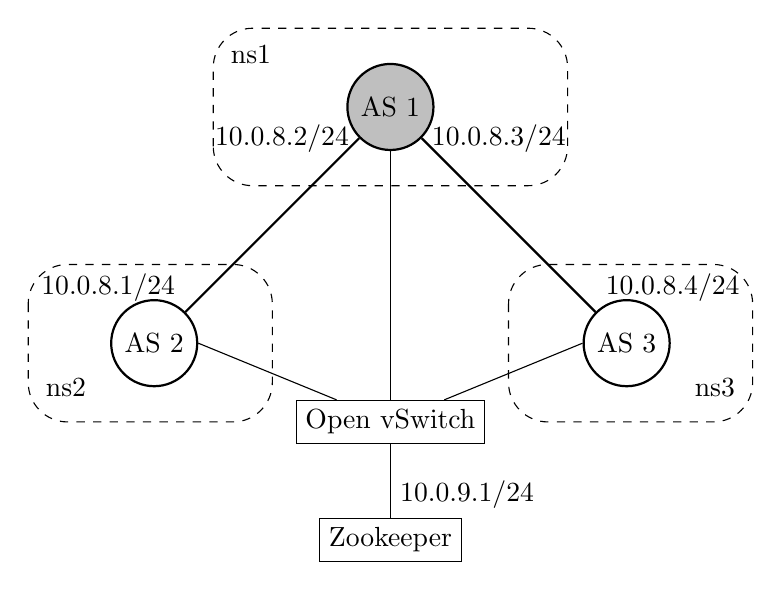
\begin{tikzpicture}
\node at (0, 0) [circle, thick, draw, fill=lightgray] (AS1) {AS 1};
\node at (-3cm, -3cm) [circle, thick, draw] (AS2) {AS 2};
\node at (3cm, -3cm) [circle, thick, draw] (AS3) {AS 3};

\node at (0cm, -4cm) [rectangle, draw] (OVS) {Open vSwitch};
\node at (0cm, -5.5cm) [rectangle, draw] (zookeeper) {Zookeeper};

\draw[thick] (AS1.south west) node[anchor=east] {10.0.8.2/24} -- (AS2.north east) node[anchor=south east] {10.0.8.1/24};
\draw[thick] (AS1.south east) node[anchor=west] {10.0.8.3/24} -- (AS3.north west) node[anchor=south west] {10.0.8.4/24};

\draw[thin, dashed, rounded corners=5mm] (-2.25cm, -1cm) rectangle (2.25cm, 1cm);
\node at (-2.15cm, 0.9cm) [anchor=north west] {ns1};
\draw[thin, dashed, rounded corners=5mm] (-4.6cm, -2cm) rectangle (-1.5cm, -4cm);
\node at (-4.5cm, -3.8cm) [anchor=south west] {ns2};
\draw[thin, dashed, rounded corners=5mm] (1.5cm, -2cm) rectangle (4.6cm, -4cm);
\node at (4.5cm, -3.8cm) [anchor=south east] {ns3};

\draw[thin] (AS1.south) -- (OVS);
\draw[thin] (AS2.east) -- (OVS);
\draw[thin] (AS3.west) -- (OVS);
\draw[thin] (zookeeper.north) node[anchor=south west] {10.0.9.1/24} -- (OVS);
\end{tikzpicture}
\caption{SCION topology}
\label{fig:topology}
\end{figure}

%%%%%%%%%%%%%%%%%%%%%%%%%%%%%%%

\section{Switch Fabric APIs}
There are a number of open APIs provided by the switch silicon vendors. In case of Broadcom there are four libraries that seemed useful to our project: OpenNSL, OF-DPA, SAI, and SDKLT. In the following we briefly introduce each one and explain why we mostly used OpenNSL.

\paragraph{OpenNSL (Open Network Switch)}
OpenNSL provides a collection of APIs to configure and monitor switching ASICs. There are APIs to control port settings, gather statistics and control L2 switching and L3 routing tables. Depending on hardware support, features like VLANs, QoS, trunking, tunneling, MPLS, and others can be accessed. There is also a warm boot feature that allows the control plane software to restart without disrupting the data plane. The following APIs were of particular interest to us:
\begin{description}
\item [Packet Tx/Rx] OpenNSL can receive packets on the CPU and sent packets from the CPU out one of the switch ports. This has the potential to speed up the SCION border router by bypassing the Linux network stack and communicating more directly with the hardware.
\item [Kernel Network (KNET)] Packet transmission and reception can be handled by a kernel module providing virtual network interfaces visible to the OS. This makes the switch ports accessible like any other network interface. Additionally KNET allows to set filters that de-multiplex received packets to one of the virtual interfaces or the Tx API depending on a range of conditions. The knet filters are able to match arbitrary packet data, potentially enabling us to match hop fields in the SCION packet header. The filtering is done purely in software however.
\item [Field Processor] The field processor API allows us to configure packet header matching in hardware. It can set rules to classify packets and take appropriate actions on them like forwarding a packet to a certain port or dropping it. The OpenNSL documentation indicates it might be possible to match arbitrary user-defined header fields\footnote{\url{http://broadcom-switch.github.io/OpenNSL/doc/html/OPENNSL_FIELD_PROCESSOR_OVERVIEW.html}}, but we did not find the appropriate functionality in the documented API.
\end{description}

OpenNSL is distributed in two versions. There is the ``Community Development Package'' available on GitHub\footnote{\url{https://github.com/Broadcom-Switch/OpenNSL}} and the ``OEM/ODM Development Package'' only available to Broadcom's customers under a license agreement. The open Community Development Package only contains the C headers declaring the interface, but not the source code of OpenNSL itself which is only included in the OEM/ODM package. Therefore we rely on the switch manufacturer to provide suitable binaries for the operating system we are running. It is worth noting that the same OpenNSL binary can be used on multiple platforms by supplying it with a matching configuration file. More information is available in the OpenNSL white paper\footnote{\url{https://docs.broadcom.com/docs/12378910}}.

Even though the source code of the user mode components of OpenNSL is not available, the GPL-licensed source code of the kernel modules it requires, is. This gives us some more flexibility in choosing a network operating system, since we can compile the modules for a different kernel version than the one supported by the manufacturer of the switch. Our efforts to compile the kernel modules for Open Network Linux are documented in Section~\ref{sec:kernel_modules}.

\paragraph{OF-DPA (OpenFlow Data Plane Abstraction)}
OF-DPA is a C API enabling implementation of OpenFlow~1.3.4. It uses the same software infrastructure as OpenNSL and is distributed in a similar way with a community and an OEM/ODM package. The API specification and a reference implementation of an OpenFlow agent build on OF-DPA are available on GitHub\footnote{\url{https://github.com/Broadcom-Switch/of-dpa}}.

We considered OF-DPA since the ``extensible match'' format used to specify packet match rules since OpenFlow~1.2 allows for ``experimenter'' extensions that might have given us a way around limitations of the OpenNSL field processor API. The OF-DPA specification\footnote{\url{https://github.com/Broadcom-Switch/of-dpa/blob/master/OFDPAS-ETP100-R.pdf}} defines a number of experimenter header fields, but does not introduce user-defined header fields limiting OF-DPA's use for us. Nevertheless we implemented a small application to explore the API, see Section~\ref{sec:ofdpa_test_app}.

\paragraph{SAI (Switch Abstraction Interface)}
The Switch Abstraction Interface is a vendor-independent API under the umbrella of the Open Compute Project\footnote{\url{https://github.com/opencomputeproject/SAI}}. Broadcom's implementation\footnote{\url{https://github.com/Broadcom-Switch/SAI}} seems to be a wrapper around OpenNSL and is not available for the switches we used in this project, hence we did not investigate it further.

\paragraph{SDKLT (Logical Table Software Development Kit)}
SDKLT has a similar aim to OpenNSL in that it allows the community to build and test software for Broadcom switching devices without a license agreement, but it exposes a different style of API focused on ``logical tables''. Logical tables provide an abstraction of physical forwarding tables installed in the device. Like in OpenNSL there is the possibility to send and receive packets from the CPU including KNET functionality. Interestingly a low-level API providing direct access to the physical tables and chip registers is also documented. SDKLT's source code is publicly available\footnote{\url{https://github.com/Broadcom-Network-Switching-Software/SDKLT}}, It is in part licensed under the Apache 2.0 license and in part under the Broadcom Switch Software license. Currently the only supported ASIC is the Broadcom BCM56960 Tomahawk but a control plane simulator is included.

\subsection{Library Versions and Development Environment}
We used the headers and examples of OpenNSL version 3.5.0.1 (commit \texttt{eb1cfd0}) and OF-DPA version 2.02 (commit \texttt{7c4b5f2}) for testing and development. The corresponding binaries for Open Network Linux were supplied by Edgecore. We build example applications and our own code on the switches themselves and under Ubuntu 16.04 using the native x86-64 gcc toolchain and the arm-linux-gnueabi ARM-toolchain.

%%%%%%%%%%%%%%%%%%%%%%%%%%%%%%%

\subsection{Compiling the OpenNSL examples}
The OpenNSL distribution on GitHub includes a number of example applications. To compile them we edited the provided makefile to use the \texttt{libopennsl} binaries provided by Edgecore. Compiling for the x86 based AS5812 worked without issues. On the ARM based AS4610 however, we encountered a linker error because of two missing symbols. The symbols in question are \texttt{bcm\_ether\_atoe} and \texttt{bcm\_ether\_ntoa}. These symbols are imported by the \texttt{libopennsl} provided by Edgecore, but no other library provides them. Instead they are defined in the precompiled examples included with this \texttt{libopennsl}, but are not mentioned in the source code we have for the examples. There is a slight version mismatch between the source code provided on GitHub (3.5.0.1) and the binaries (3.5.0.3) that might explain the difference, though the x86 binaries do not contain the problematic symbols.

\texttt{bcm\_ether\_atoe} and \texttt{bcm\_ether\_ntoa} refer to two functions converting between binary and textual representations of MAC addresses. We found these functions in source code published by Broadcom not directly related to OpenNSL. As a stopgap solution we can compile the examples and our own applications by linking in these functions.

%%%%%%%%%%%%%%%%%%%%%%%%%%%%%%%

\subsection{Compiling the OpenNSL kernel modules} \label{sec:kernel_modules}
OpenNSL requires three loadable kernel modules in order to communicate with the switching hardware. These modules are called \texttt{linux-kernel-bde}, \texttt{linux-user-bde}, and \texttt{linux-bcm-knet}. The former two are required by most parts of the API, the last one is only necessary for the kernel networking feature. \texttt{linux-user-bde} and \texttt{linux-bcm-knet} depend on \texttt{linux-kernel-bde}, so \texttt{linux-kernel-bde} must always be loaded first.

The source code of these modules is included in the GitHub repository under \texttt{sdk-6.5.12-gpl-modules}. Since no prebuild modules were available for the armhf port of Debian, we tried to compile them ourselves. The first step was to compile for the x86-64 architecture and Linux kernel version 4.4.0-98 using a makefile provided by Broadcom.

\begin{lstlisting}[language=bash]
sudo apt-get install linux-headers-4.4.0-98-generic
cd OpenNSL/sdk-6.5.12-gpl-modules/systems/linux/user/x86-smp_generic_64-2_6
export platform=x86-smp_generic_64-2_6
export ARCH=x86
export KERNDIR=/lib/modules/4.4.0-98-generic/build/
export LINUX_INCLUDE=/lib/modules/4.4.0-98-generic/build/include/
make
\end{lstlisting}

The modules built successfully. Next we tried to cross-compile for ARM and ONL kernel version \texttt{4.14.49-OpenNetworkLinux-armhf}. Naturally there is no makefile for this specific configuration in the repository, but there are makefiles for Broadcom's iProc family of of SoCs. Unfortunately we were not able to use them directly, because they are made for older versions of the Linux kernel and are probably not targeted at the specific chip in the switch we used. Instead we combined parts of the x86 makefiles we knew were working and the ARM makefiles. Additionally we had to make some small changes to accommodate the newer kernel version. The complete makefiles we used are in Appendix~\ref{app:kernel_module_makefiles}.

After installing the kernel source code from a deb package created during the ONL build process, the makefiles are invoked as follows:

\begin{lstlisting}[language=bash, breaklines=true]
cd OpenNSL/sdk-6.5.12-gpl-modules/systems/linux/user/arm
export KERNDIR=/usr/share/onl/packages/armhf/onl-kernel-4.14-lts-armhf-iproc-all/mbuilds
make ARCH=arm CROSS_COMPILE=arm-linux-gnueabihf-
\end{lstlisting}

With these changes we were still not able to compile the modules successfully. We additionally had to make some modifications to the source code: We replaced the deprecated function \texttt{pci\_enable\_msix} with \texttt{pci\_enable\_msix\_exact} and upgraded code accessing a removed member of the \texttt{net\_device} struct. The exact changes are listed in Appendix~\ref{app:kernel_modules}.

With these modifications the modules built successfully but the modules failed to load with a failing assertion. We traced the problem to a call to \texttt{cma\_alloc()} failing that would allocate contiguous memory for DMA. Reducing the amount of memory set aside for DMA enabled the modules to load successfully.

\begin{lstlisting}[language=bash]
sudo insmod linux-kernel-bde.ko dmasize=2M
sudo insmod linux-user-bde.ko
sudo insmod linux-bcm-knet.ko
\end{lstlisting}

Unfortunately the \texttt{linux-kernel-bde} we compiled fails to detect the switching hardware. The BCM56340 Helix4 chip used in the AS4610 switch is mentioned in the source code, so it probably should be supported. By passing the parameter \texttt{debug=5} to \texttt{linux-kernel-bde} we were able to find a failing call to \texttt{pci\_find\_bus(0,0)} that should find the PCI root bus. This might indicate that we failed to correctly configure the source code for the chip we were using. We did not investigate further, since we ultimately decided to abandon the armhf port in favor of the officially supported armel.

%%%%%%%%%%%%%%%%%%%%%%%%%%%%%%%

\subsection{OpenNSL Test Application} \label{sec:opennsl_test_app}
To get familiar with OpenNSL and to configure the virtual network interfaces we could use to run a local SCION topology we developed an application accessing the KNET and some of the port configuration and monitoring features of OpenNSL. Additionally we included support for sending and receiving test packets from the CPU. We based our program on the examples \texttt{example\_knet.c}, \texttt{example\_stat.c}, and \texttt{example\_packet\_transmit.c} in the \texttt{examples} directory of OpenNSL's source repository. We included instructions on how to build the application in the source code archive that comes with this document.

Note that in general only a single application can use OpenNSL at the same time and that initializing the library resets all switching chips in the system to their default state. This also extends to other libraries that access the hardware like OF-DPA. They can not run in parallel with an OpenNSL application. A problem we faced with KNET in this regard and one of the reasons to write our own program is that the virtual network interfaces created by OpenNSL are, at least in our case, not automatically removed. The KNET example application included with OpenNSL cannot remove interfaces created by previous instances of itself, so we had to write this functionality ourselves.

When our test application starts, it puts every Ethernet port on the switch in its own VLAN. All ports are set to send packets without a VLAN tag and treat received packets as if they belong to their own VLAN. The CPU port is added to all VLANs. Having the ports in different VLANs is necessary to prevent a packet from being endlessly send back and forth if two ports are looped with a cable.

\paragraph{Usage Examples}
In the following we present some usage examples. After invoking our test program, the user is presented with a prompt. An empty command string displays a list of valid commands.

List all switch ports:
\begin{lstlisting}
>ls port
Port  1: enabled, speed: 1000 Mbps
Port  2: enabled, speed: 0 Mbps
Port  3: enabled, speed: 10000 Mbps
Port  4: enabled, speed: 10000 Mbps
...
\end{lstlisting}

Get port statistics:
\begin{lstlisting}
>stats 1
Ingress Unicast packets........ 0
Ingress Non-unicast packets.... 0
...
\end{lstlisting}

Map port 1 to a virtual network interface called ``port1'':
\begin{lstlisting}
>add netif 1 port 1
Created interface port ID: 1
Created filter port ID: 2
>ls netif
ID: 1, Port: 1, VLAN: 0, Name: "port", MAC: 02:10:18:00:00:01
>ls filter
ID: 2, Priority: 100, Ingress port: 1, DestID: 1, Description: "port"
ID: 1, Priority: 255, Ingress port: 0, DestID: 0, Description: "DefaultRxAPI"
\end{lstlisting}

Create a filter matching the byte 0x2C at offset 100 in the raw packet data:
\begin{lstlisting}
>add raw_filter 1 1 filter 100 2C FF
Created filter filter ID: 3
\end{lstlisting}
Note that the packet always contains a VLAN tag on the switch, thus potentially offsetting the rest of the fields by four bytes.

Send five test packets out port 2:
\begin{lstlisting}
>tx 2 5
Packet(s) sent
\end{lstlisting}

%%%%%%%%%%%%%%%%%%%%%%%%%%%%%%%

\subsection{OF-DPA Test Application} \label{sec:ofdpa_test_app}
We have also written an application to explore OF-DPA. Build instructions are included with the source code. Note that in contrast to OpenNSL most parts of OF-DPA do not require root privileges, but registering a callback to receive packets does. Since our applications can receive packets on the CPU it has to be run with \texttt{sudo} or appropriate permissions have to be set.

\paragraph{Usage Examples}
List flow tables:
\begin{lstlisting}
>ls table
Table   0: Ingress Port (0 / 2000)
Table   5: Port DSCP Trust (0 / 8127)
Table   6: Port PCP Trust (0 / 1023)
Table  10: VLAN (0 / 12288)
...
\end{lstlisting}

Print up to the first 10 entries of table 60:
\begin{lstlisting}[breaklines=true]
>dump table 60 10
Table  60: ACL Policy
Entries: 1 / 3840
Entry 0:  inPort:mask = 1:0xffffffff srcMac:mask = 0000.0000.0000:0000.0000.0000 destMac:mask = 0000.0000.0000:0000.0000.0000 etherType:mask = 0x0000:0x0000 | GoTo = 0 (None) outPort = CONTROLLER (Reserved)  | priority = 0 hard_time = 0 idle_time = 0 cookie = 0
\end{lstlisting}

Set up a flow table entry to send all packets on port 1 to the CPU and receive up to 10 packets:
\begin{lstlisting}[breaklines=true]
>add flow rx 1
>rx 10
Received packet on port 1, reason: 1, size: 60
0x0000  ff ff ff ff ff ff 82 2f 2e 42 46 74 08 06 00 01 08 00 06 04 00 01 82 2f 2e 42 46 74 0a 00 00 01
0x0020  00 00 00 00 00 00 0a 00 00 02 00 00 00 00 00 00 00 00 00 00 00 00 00 00 00 00 00 00
No more packets available
\end{lstlisting}

%%%%%%%%%%%%%%%%%%%%%%%%%%%%%%%

\section{Conclusion}
Current scenario of networking infrastructure requires a secure and reliable network. SCION as a first clean slate internet architecture can be an improvement for a stable and cheaper solution for network infrastructure. So to achieve a running SCION installation in a bare metal switch, we firstly loaded the open source NOS Open Network Linux. Secondly, to control the packet forwarding hardware, Broadcom's OpenNSL API was installed. Finally we were able to run SCION on a bare-metal switch. This report also presented our experiences with Broadcom's switch fabric APIs. Applying them to packet forwarding in SCION remains for future work.

%%%%%%%%%%%%%%%%%%%%%%%%%%%%%%%

\appendix
\section{Appendix}
\lstset{breaklines=true, basicstyle=\footnotesize}

\subsection{Installation of SCION on Debian 8}
\lstinputlisting[language=bash, caption={install\_scion.sh}]{source_code/install_scion/debian8/install_scion.sh}

\subsection{Makefiles for OpenNSL kernel modules} \label{app:kernel_module_makefiles}
\lstinputlisting[language=make, caption={systems/linux/user/arm-4\_4}]{source_code/opennsl_kernel_modules/arm-4_4/Makefile}
\lstinputlisting[language=make, caption={make/Makefile.linux-arm-4\_4}]{source_code/opennsl_kernel_modules/make/Makefile.linux-arm-4_4}
\lstinputlisting[language=make, caption={make/makefile.linux-arm-common-4\_4}]{source_code/opennsl_kernel_modules/make/makefile.linux-arm-common-4_4}
\lstinputlisting[language=make, caption={make/Makefile.linux-arm-generic-common-4\_4}]{source_code/opennsl_kernel_modules/make/Makefile.linux-arm-generic-common-4_4}

\subsection{Modifications to OpenNSL kernel modules} \label{app:kernel_modules}
\begin{lstlisting}[caption={systems/bde/linux/kernel/linux-kernel-bde.c}]
@@ -1973,13 +1973,13 @@ _msi_connect(bde_ctrl_t *ctrl)
         for (i = 0; i < ctrl->msix_cnt; i++)
                 ctrl->entries[i].entry = i;

-        ret = pci_enable_msix(ctrl->pci_device,
+        ret = pci_enable_msix_exact(ctrl->pci_device,
                                            ctrl->entries, ctrl->msix_cnt);
         if (ret > 0) {
             /* Not enough vectors available , Retry MSI-X */
             gprintk("Retrying with MSI-X interrupts = %d\n", ret);
             ctrl->msix_cnt = ret;
-            ret = pci_enable_msix(ctrl->pci_device,
+            ret = pci_enable_msix_exact(ctrl->pci_device,
                                            ctrl->entries, ctrl->msix_cnt);
             if (ret != 0)
                 goto er_intx_free;
\end{lstlisting}

\begin{lstlisting}[caption={systems/bde/linux/kernel/linux\_dma.c}]
@@ -873,7 +873,7 @@ _sinval(int d, void *ptr, int length)
 #if defined(dma_cache_wback_inv)
      dma_cache_wback_inv((unsigned long)ptr, length);
 #else
-#if defined(IPROC_CMICD) || defined(BCM958525)
+#if defined(IPROC_CMICD) || defined(BCM958525) || defined(__arm__)
     /* FIXME: need proper function to replace dma_cache_sync */
     dma_sync_single_for_cpu(NULL, (unsigned long)ptr, length, DMA_BIDIRECTIONAL);
 #else
@@ -889,7 +889,7 @@ _sflush(int d, void *ptr, int length)
 #if defined(dma_cache_wback_inv)
     dma_cache_wback_inv((unsigned long)ptr, length);
 #else
-#if defined(IPROC_CMICD) || defined(BCM958525)
+#if defined(IPROC_CMICD) || defined(BCM958525) || defined(__arm__)
     /* FIXME: need proper function to replace dma_cache_sync */
     dma_sync_single_for_cpu(NULL, (unsigned long)ptr, length, DMA_BIDIRECTIONAL);
 #else
\end{lstlisting}

\begin{lstlisting}[caption={systems/bde/linux/user/kernel/linux-user-bde.c}]
@@ -34,6 +34,7 @@
 #include <shared/et/bcmdevs.h>
 #endif

+#include <linux/uaccess.h>

 MODULE_AUTHOR("Broadcom Corporation");
 MODULE_DESCRIPTION("User BDE Helper Module");
\end{lstlisting}

\begin{lstlisting}[caption={systems/linux/kernel/modules/bcm-knet/bcm-knet.c}]
@@ -70,6 +70,8 @@
 #include <linux/random.h>
 #include <linux/seq_file.h>
 #include <linux/if_vlan.h>
+#include <linux/signal.h>
+#include <linux/sched/signal.h>


 MODULE_AUTHOR("Broadcom Corporation");
@@ -4771,7 +4773,8 @@ bkn_tx(struct sk_buff *skb, struct net_device *dev)
         bkn_suspend_tx(sinfo);
     }

-    dev->trans_start = jiffies;
+    // dev->trans_start = jiffies;
+    netdev_get_tx_queue(dev, 0)->trans_start = jiffies;

     spin_unlock_irqrestore(&sinfo->lock, flags);
\end{lstlisting}

\end{document}
